The MAW app is split into two major components. The first is a pathway browser
that adds tissue and compartment information to the individual pathways. The
second is a touch-based implementation of the SMDA (Steady-State Metabolic
Network Dynamics Analysis) tool.

\section{Pathway Browser}

The iPad application displays metabolic pathway graphs for all pathways for
which PathCase provides a static layout. These graphs can be navigated by
panning and zooming.

\subsection{Interface}
\label{sect:maw_interface}

The home screen of \mawapp displays a list of pathways that the user can choose
from to view a graph. This screen is shown in figure
\ref{fig:maw_screenshot_list}. It also contains a brief explanation of the
PathCase database and instructions for using \mawapp. The button in the bottom
left corner activates the SMDA tool, described in section \ref{sect:smda}.

\begin{figure}[htbp]
    \center{
        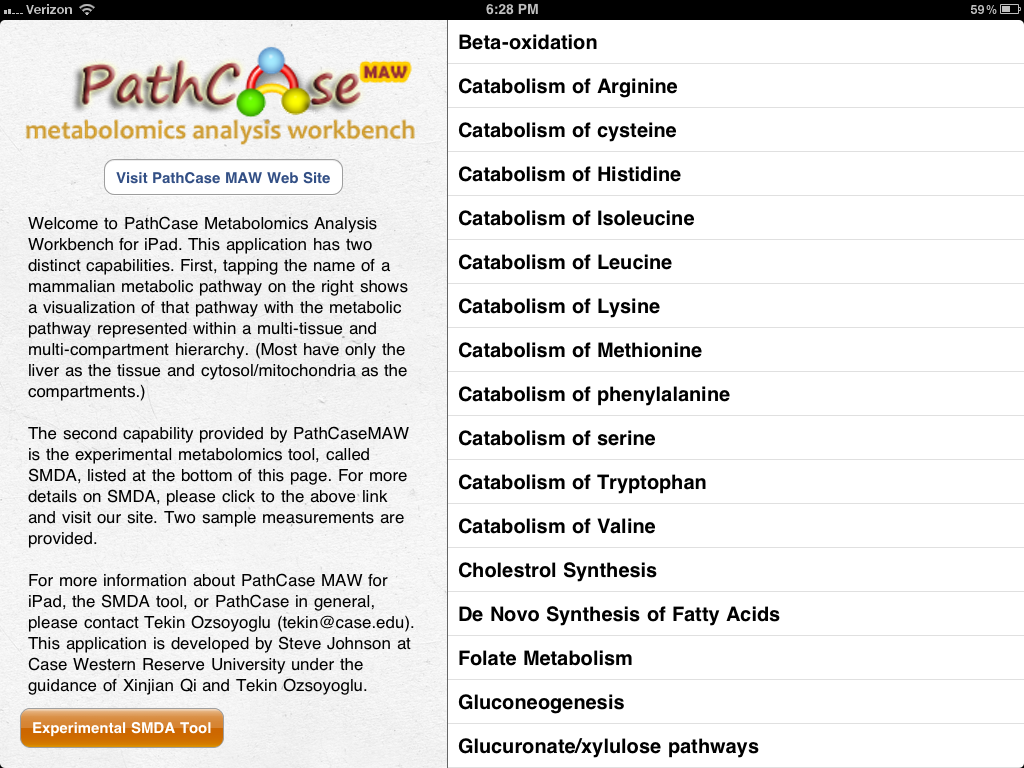
\includegraphics[width=4.5in]{maw/figures/screenshot_list}}
    \caption{\label{fig:maw_screenshot_list} List of pathways on the main screen
    of \mawapp}
\end{figure}

\begin{figure}[hbtp]
    \center{
        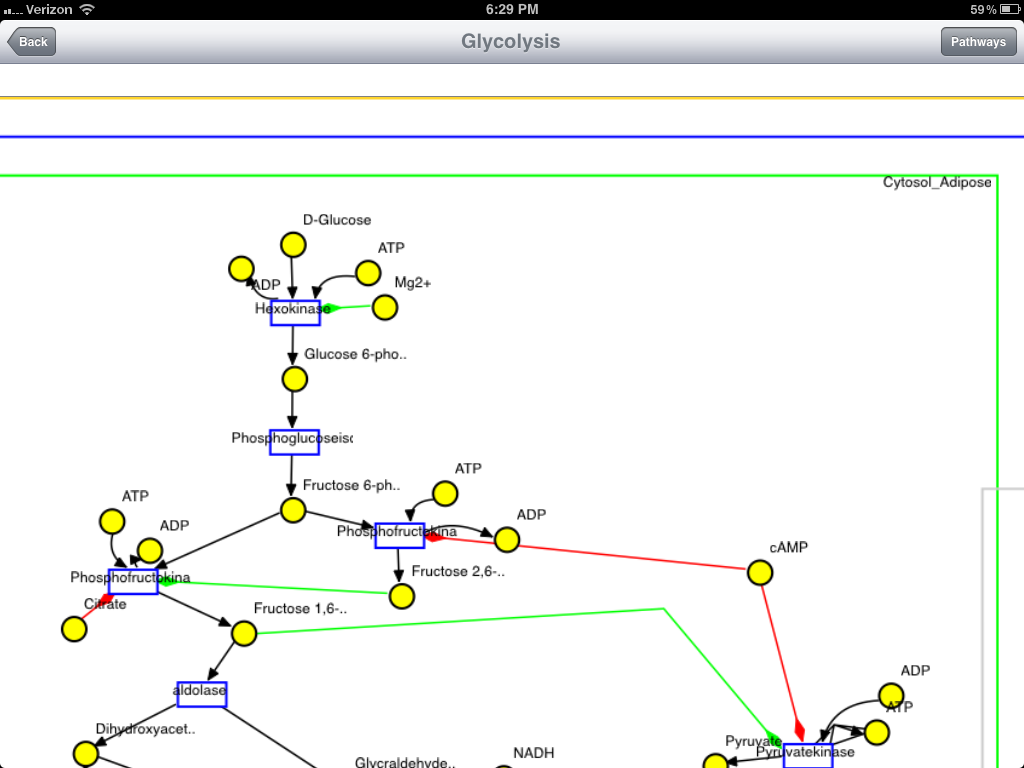
\includegraphics[width=4.5in]{maw/figures/screenshot_glycolysis}}
    \caption{\label{fig:maw_screenshot_pathway} Compartment-aware visualization
    of Glycolysis}
\end{figure}

After selecting a pathway by tapping a row in the list, the user enters the
pathway visualization. In this screen, they can drag across the screen with one
finger to move the view. They can use two fingers in a pinching motion to zoom
in or out. The view for glycolysis is shown in figure
\ref{fig:maw_screenshot_pathway}.

The pathway visualization consists of several components. The most important are
the nodes in the graph. The rectangular nodes represent reactions. The rest of
the nodes represent metabolites. The edges represent relationships such as
product, substrate, cofactor, or inhibitor. The rectangular outlines around
sections of the graph represent the compartment that the pathway is classified
under.

In figure \ref{fig:maw_screenshot_pathway}, Glycolysis is displayed in two
different compartments: $Organs \rightarrow Blood \rightarrow Cytosol\_Adipose$
and $Organs \rightarrow Blood \rightarrow Cytosol\_Liver$. These compartments
are shown using nested rectangles with text labels in the upper right corner.

\begin{figure}[hbtp]
    \center{
        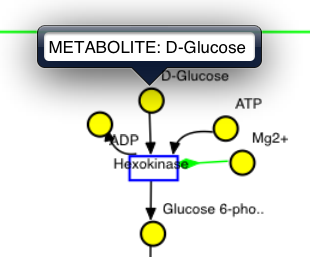
\includegraphics[width=3in]{maw/figures/screenshot_glycolysis_popover}}
    \caption{\label{fig:maw_screenshot_popover} Tapping a node displays a
    popover with the node's full name}
\end{figure}

When a node is tapped, a popover appears with the full name of the object
represented by the nodes, as well as any relevant relationships or other
information. Figure \ref{fig:maw_screenshot_popover} demonstrates this behavior.


\subsection{Implementation}
\label{sect:maw_implementation}

The MAW application must track a few different categories of data. The most
basic is a representation of the data model of the online PathCase MAW database,
derived from the web service interface to the database. Examples include
pathways, metabolites, compartments, and processes. In Model-View-Controller
terms (see \ref{sect:implementation_notes}), these are \textbf{model} classes.
These model objects are rendered in \textbf{views}, such as the main pathway
graph view.  These views are managed by \textbf{controllers} which manipulate
the models and configure the views.

The relationships between some of the major classes of the PathCase MAW app are
represented in three figures. Figure \ref{fig:maw_components} shows references
between instances. Figure \ref{fig:maw_controlflow} shows the flow of control in
response to events from the event loop. Figure \ref{fig:maw_dataflow} shows the
flow of data between the methods involved in loading and displaying a graph.

\subsubsection{Data Model}
\label{sect:maw_data_model}

\subsubsection{User Interface}
\label{sect:maw_ui}

An application-level singleton, \texttt{PCAppDelegate}, handles
application-level delegate methods and notifications from the system. Another
singleton, \texttt{PCMainMenuViewController}, sits on top of
\texttt{PCAppDelegate} and displays the home screen, including the list of
pathways and button to enter SMDA.

When an item in the list of pathways is tapped, a new view is shown, controlled
by \texttt{PCPathwayNavController}. This view controller object controls the
toolbar (currently just the ``Pathways'' button) and a content area that can
contain any view and corresponding view controller.

When displaying a pathway, as is the normal case, the content area is controlled
by \texttt{PCGraphViewController}. This view controller object controls a
\texttt{PCGraphView} which, in turn, renders all nodes and edges in a scrollable
and zoomable fashion.

The Pathways button causes a popover list of available pathways to be displayed.
This popover is populated by \texttt{PCPathwayListTableController}, which
transforms pathway model objects into a form understood by the built-in table
view. When one of these pathway names is clicked, an event is sent back to the
\texttt{PCPathwayNavController}, which loads the new pathway from the device's
internal storage, builds a new \texttt{PCGraphViewController}, and inserts it in
the content area.

The graph view controller controls a \texttt{PCGraphView} which contains Core
Animation layers that read the pathway model and render the nodes and edges with
OpenGL. (See \ref{sect:implementation_notes}.) These layers are put inside the
Cocoa object \texttt{UIScrollView}, which allows them to be panned and zoomed
over by touch.

\subsubsection{Web Services}
\label{sect:maw_web_services}

Although the data is accessed via web services, it is needed so often and is
small enough that the entire database is contained within the app. The database
can be updated whenever the user chooses via the user interface.

Each web service corresponds roughly to one data type in the model, so those
model objects contain methods to load their data from the corresponding web
service. For example, the method \texttt{[PCPathway loadDataFromServer]}
updates all pathway objects. However, this method relies on some data for
tissues and metabolites to have been downloaded already, so the data update
process uses mutexes and asynchronous network requests to ensure that the data
is downloaded in the correct order while using parallelism as much as possible.

These web service fetching methods convert the XML response of the web service
into corresponding model objects (such as \texttt{SMDAPathway}) which are
serialized to the device's internal storage.

% \onecolumn

\begin{figure}[p]
    \center{
        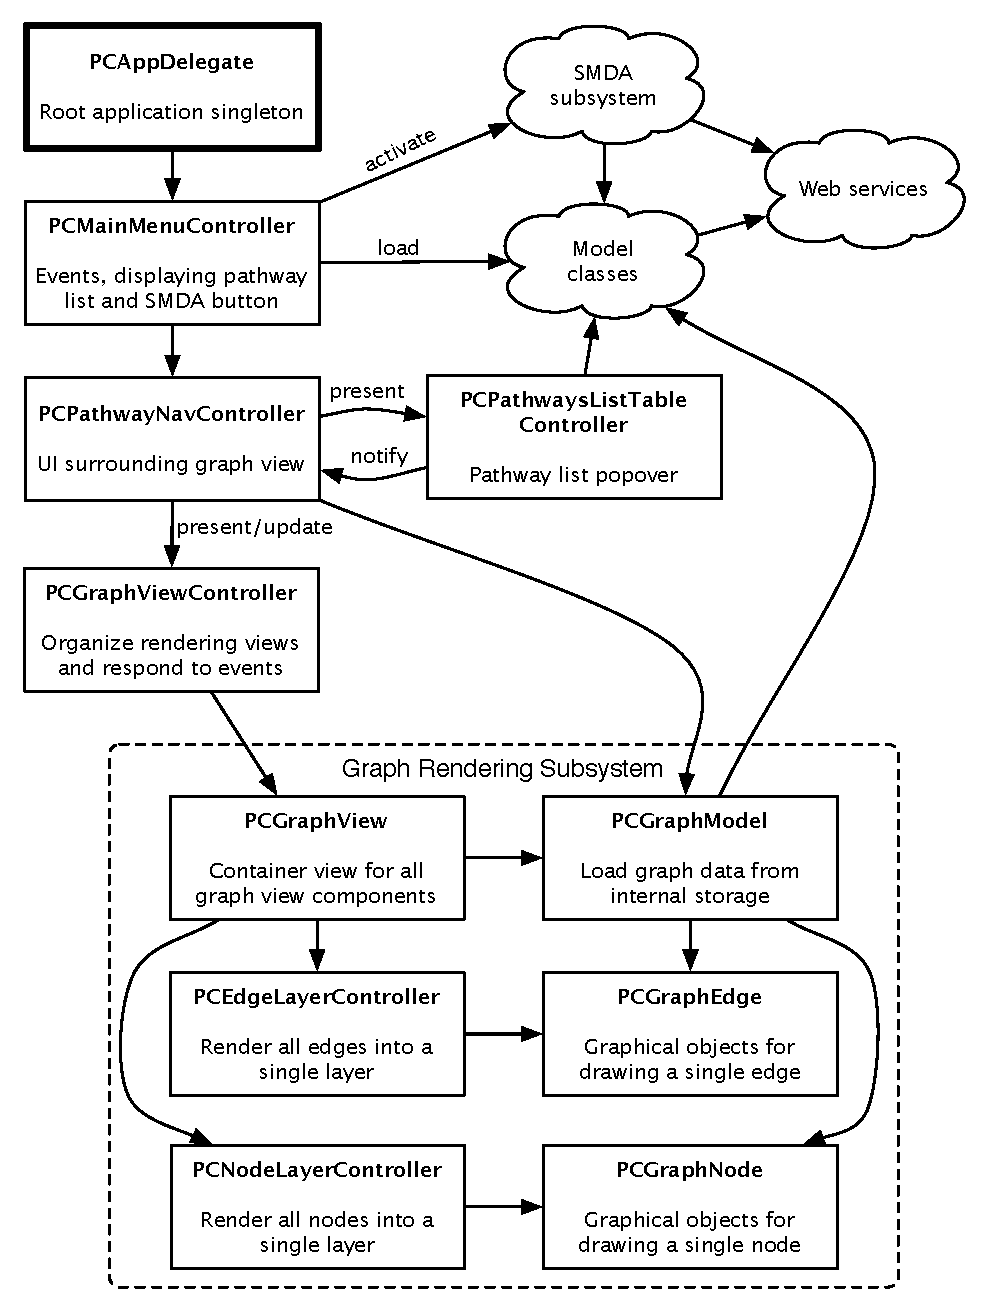
\includegraphics[width=4.5in]{maw/figures/components.pdf}}
    \caption{\label{fig:maw_components} Components of the architecture}
\end{figure}

\begin{figure}[htbp]
    \center{
        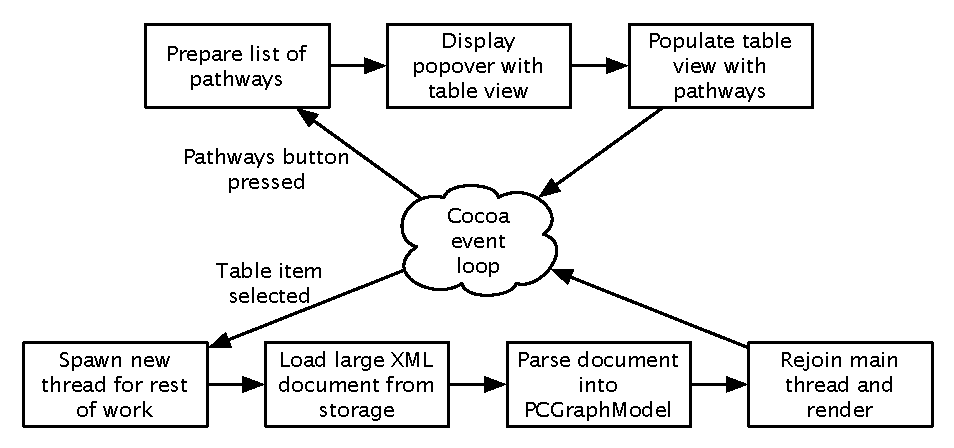
\includegraphics[height=2in]{maw/figures/controlflow.pdf}}
    \caption{\label{fig:maw_controlflow} Control flow for displaying graphs}
\end{figure}

\begin{figure}[thbp]
    \center{
        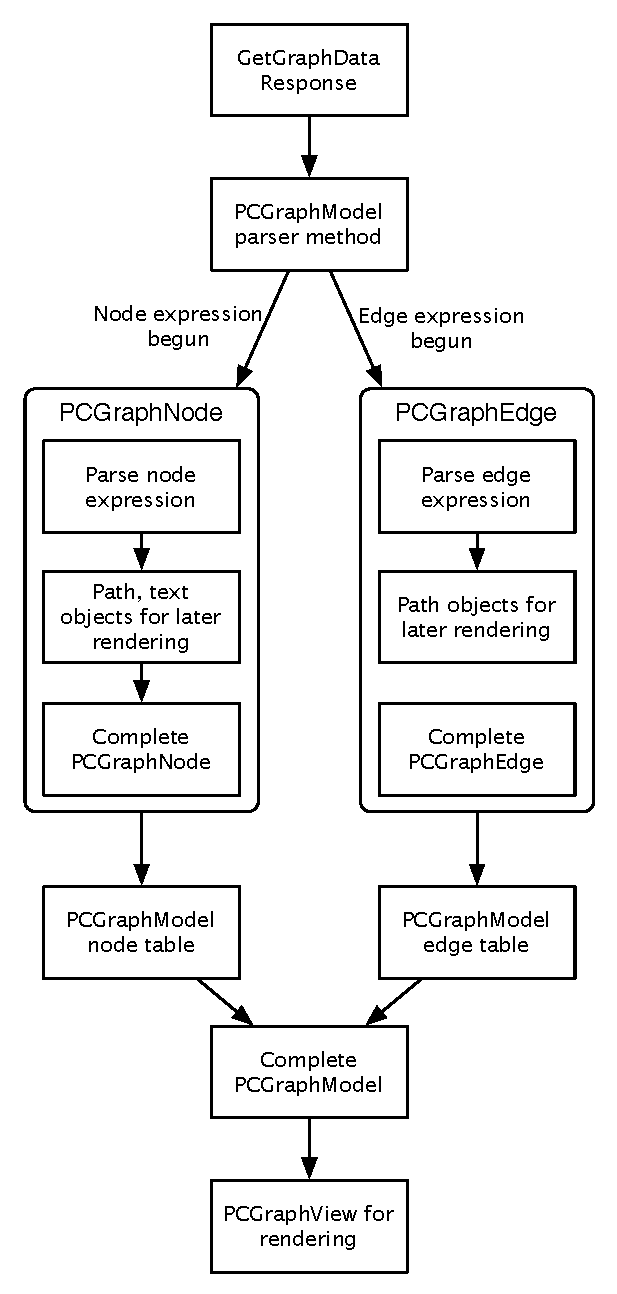
\includegraphics[height=4in]{maw/figures/dataflow.pdf}}
    \caption{\label{fig:maw_dataflow} Data flow for graph data}
\end{figure}

% \twocolumn


\section{SMDA}
\label{sect:smda}

\subsection{Interface}
\label{sect:smda_interface}

The ``Experimental SMDA Tool'' button on the home screen takes the user to a
list of measurements. \mawapp with two example result sets to help the user get
accustomed to the interface.

\subsubsection{Input}
\label{sect:smda_interface_input}

Tapping one of these measurement lists switches to the screen shown in figure
\ref{fig:screenshot_smda_list}. There is one section on this screen for each
type of input to the SMDA algorithm: pathway, transport process, reaction,
pathway as reaction, and measurement.

\begin{figure}[htb]
    \center{
        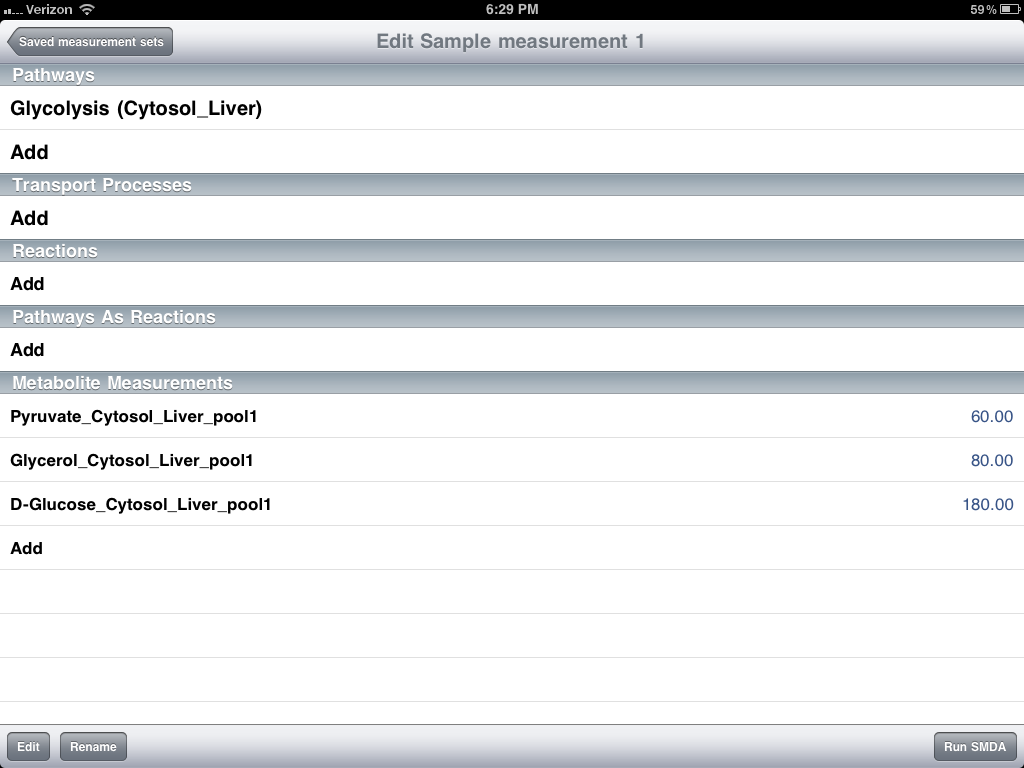
\includegraphics[width=3in]{maw/figures/screenshot_smda_list}}
    \caption{\label{fig:screenshot_smda_list} List of measurements in SMDA}
\end{figure}

\begin{figure}[htb]
    \center{
        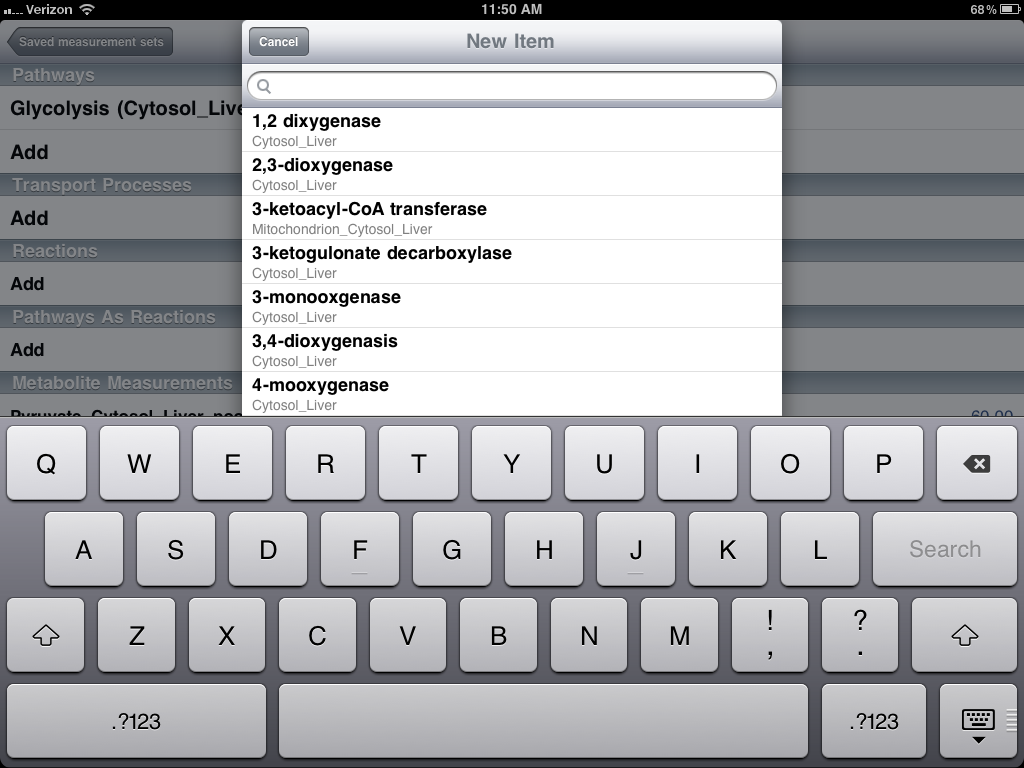
\includegraphics[width=3in]{maw/figures/screenshot_smda_add_reaction}}
    \caption{\label{fig:smda_add_reaction} Adding a reaction in SMDA}
\end{figure}

\begin{figure}[htb]
    \center{
        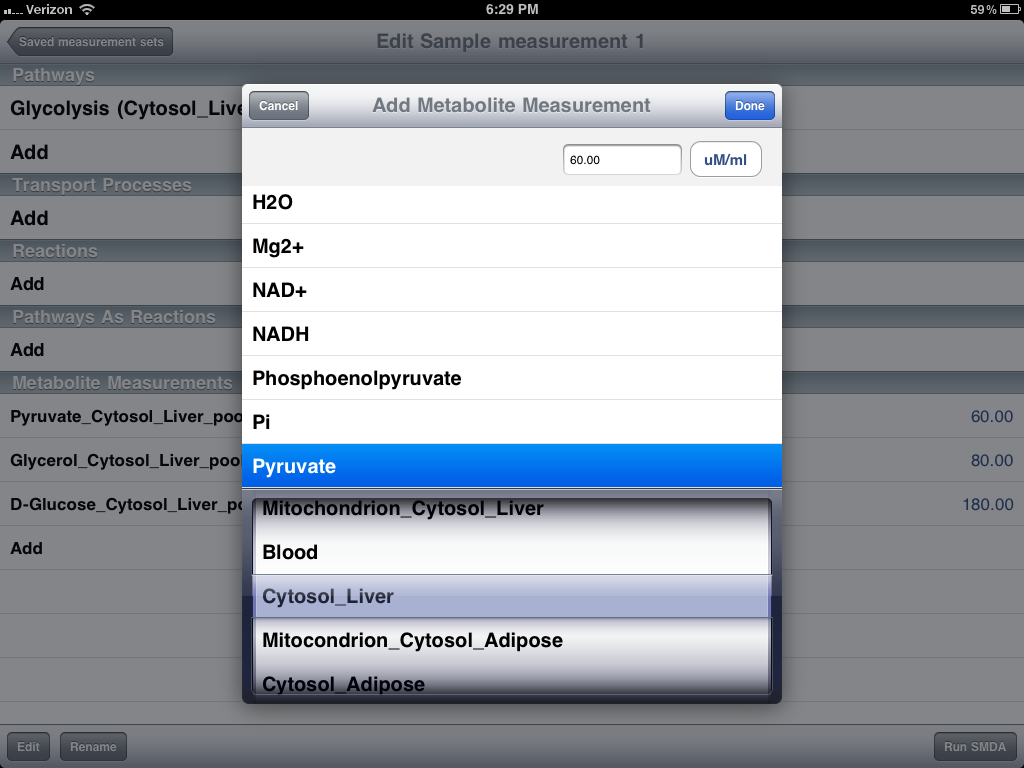
\includegraphics[width=3in]{maw/figures/screenshot_smda_edit_measurement}}
    \caption{\label{fig:smda_edit_measurement} Editing a measurement in SMDA}
\end{figure}

New input parameters can be added by tapping the ``Add'' row in any of the
sections. Figure \ref{fig:smda_add_reaction} shows the screen for adding a new
reaction. Tapping an existing row brings up the same screen, allowing the user
to change their selection.

Figure \ref{fig:smda_edit_measurement} shows a similar screen for editing
measurements.

\subsubsection{Output}
\label{sect:smda_interface_output}

The interface for browsing SMDA results is very similar to the one for looking
at a normal pathway. There are two main differences. The first, shown in figure
\ref{fig:smda_results}, is the bottom toolbar that provides buttons to move
forward and backward in the list of scenarios.

\begin{figure}[htb]
    \center{
        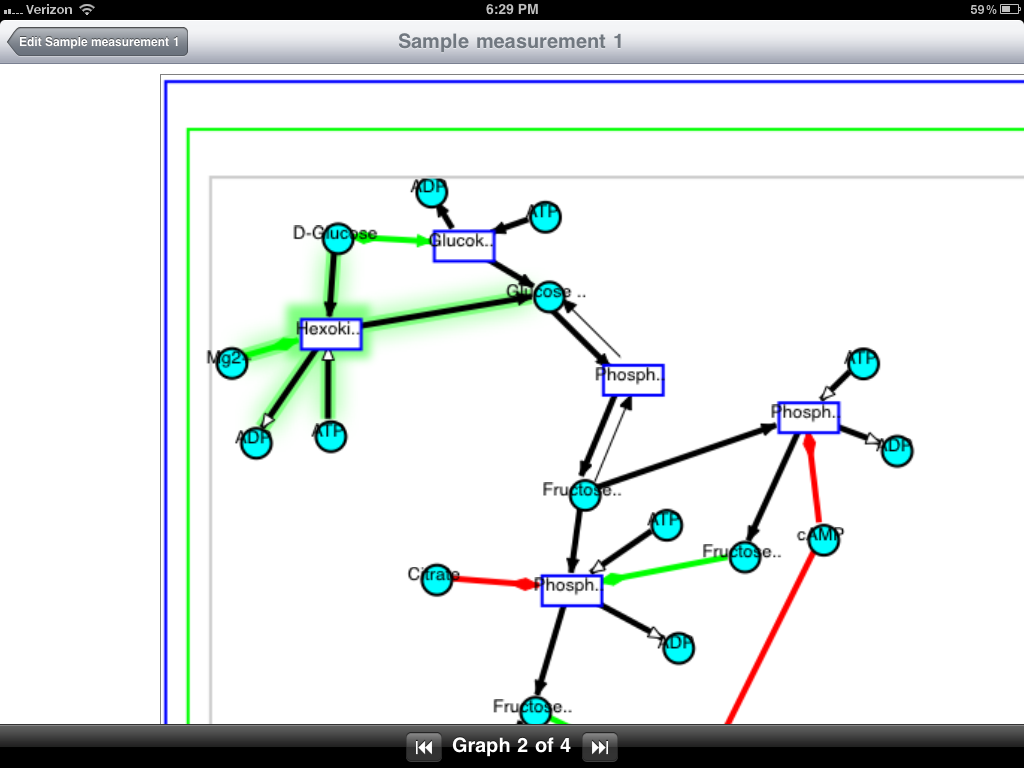
\includegraphics[width=3in]{maw/figures/screenshot_smda_results}}
    \caption{\label{fig:smda_results} One scenario in an SMDA result set}
\end{figure}

The second difference, shown in figure \ref{fig:smda_results_highlight}, is the
green highight shown behind edges coming out of a reaction if that reaction is
in a different active/inactive state from the previously viewed scenario. In
this example, ``Triose...'' was inactive in scenario 1 but active in scenario 2.
Flipping between the two scenarios will keep this reaction highlighted.

\begin{figure}[htb]
    \center{
        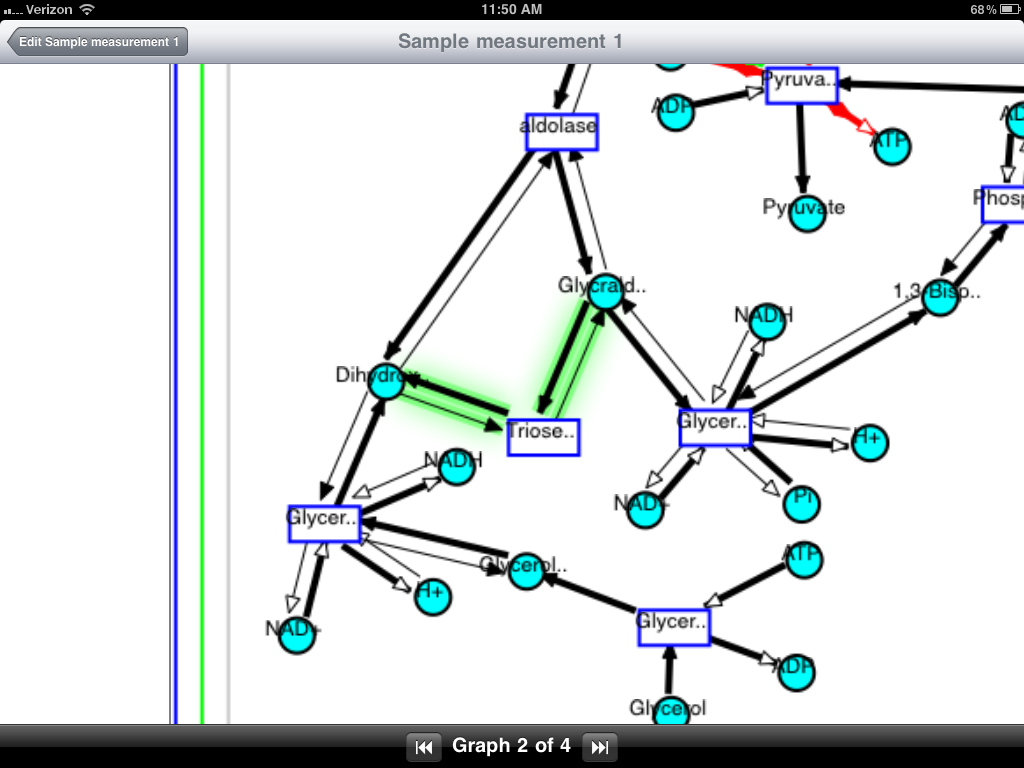
\includegraphics[width=3in]{maw/figures/screenshot_smda_results_highlight}}
    \caption{\label{fig:smda_results_highlight} Zoomed view of a highlighted
    reaction in an SMDA scenario}
\end{figure}


\section{SMDA Implementation}
\label{sect:smda_implementation}

SMDA makes full use of the \pathcasemaw data model, so \mawapp must store that
data model internally. It must store information about pathways, metabolites,
tissues, reactions, and more.

Section \ref{sect:smda_data_model} describes the subset of the \pathcasemaw data
model that is used by \mawapp to provide the SMDA tool. Section
\ref{sect:smda_web_services_server} enumerates the web services that
\pathcasemaw provides to download these model objects into \mawapp. Section
\ref{sect:smda_web_services_client} explains how \mawapp accesses these web
services and converts their results into model objects to be used by the
application.
% MORE MORE MORE

Since SMDA uses the MAW data model, it shares all model classes, with a couple
of additions. There is an \texttt{SMDASavedMeasurement} class for storing the
user's selections. There is also a subclass of \texttt{PCGraphModel} called
\texttt{SMDAResultGraphModel} which provides methods to build a model out of XML
from the web service.

The remaining classes manage the user interface. They are basic subclasses of
Cocoa objects that implement standard design patterns for iOS applications to
display the interface shown in the screenshots in section
\ref{sect:smda_interface}.

\subsection{Data Model}
\label{sect:smda_data_model}

The Objective-C classes representing the model objects use the \texttt{SMDA}
prefix, but the prefix is omitted in this section for clarity.

\begin{itemize}

    \item \textbf{Pathway}: Top level object containing all information about a
        pathway including name, identifier, 

\end{itemize}

\subsection{Web Services: Server Side}
\label{sect:smda_web_services_server}

\subsection{Web Services: Client Side}
\label{sect:smda_web_services_client}

Although the data is accessed via web services, it is needed so often and is
small enough that the entire database is distributed with the application
package in the form of serialized objects. The database can be updated whenever
the user chooses via the user interface.

Each web service corresponds roughly to one data type in the model, so those
model objects contain methods to load their data from the corresponding web
service. For example, the method \texttt{[PCPathway loadDataFromServer]}
updates all pathway objects. However, this method relies on some data for
tissues and metabolites to have been downloaded already, so the data update
process uses mutexes and asynchronous network requests to ensure that the data
is downloaded in the correct order while using parallelism as much as possible.

These web service fetching methods convert the XML response of the web service
into corresponding model objects (such as \texttt{SMDAPathway}) which are
serialized to the device's internal storage.


%%%

\section{Future Work}
\label{sect:maw_future_work}

The biggest problem with the current architecture of \mawapp is its complex
system for downloading and saving the SMDA database via the web services. The
acts of making HTTP requests, parsing them, building model objects, and
serializing those objects are entangled in a handful of functions with poor
encapsulation. These concerns should be separated and a more discrete pipeline
should be constructed.

It may be beneficial to store all data model objects in a SQLite database
instead of as serialized Objective-C objects so that they can be interacted with
in a way that more closely parallels the rest of the \pathcasemaw system.

The SMDA input interface, while functional, is somewhat cumbersome to work with.
Any given input operation requires at least three taps and lots of dragging to
complete. One possibility is that \mawapp could download a spreadsheet
containing the data from Dropbox or the user's email inbox.

As explained in section \ref{sect:smda_results_request}, the SMDA results
browser is currently unable to deal with measurements that include more than one
pathway because it cannot generate dynamic layouts. Now that Graphviz has been
added to \keggapp, it should be possible to include that functionality in
\mawapp and provide support for measurements with more than one pathway.

The original SMDA paper by Cakmak et al \cite{smda-basic} mentions that the
number of results is exponential based on the number of measurements. It might
be helpful to add a ``star'' button to the results browsing toolbar to allow a
user to mark a hypothesis that looks particularly promising, and display all
starred hypotheses in a menu.

Another improvement would be to allow the user to export his results to some
externally readable format such as PDF. The iOS application frameworks make PDF
rendering relatively simple. Combined with the ability to ``star'' hypotheses,
this could be a good way for researchers to communicate interesting SMDA
findings.

